Here we consider 3-periodics inscribed in a unit circle and circumscribing a non-concentric ellipse. We will work in the complex plane and apply Blaschke Products described in \cite{daepp-2019}, whereby Poncelet 3-periodic vertices become symmetric with respect to the information of the circle-ellipse pair. These were first used to analyze loci of Poncelet triangle centers in \cite{helman2021-power-loci}.

\begin{figure}
    \centering
    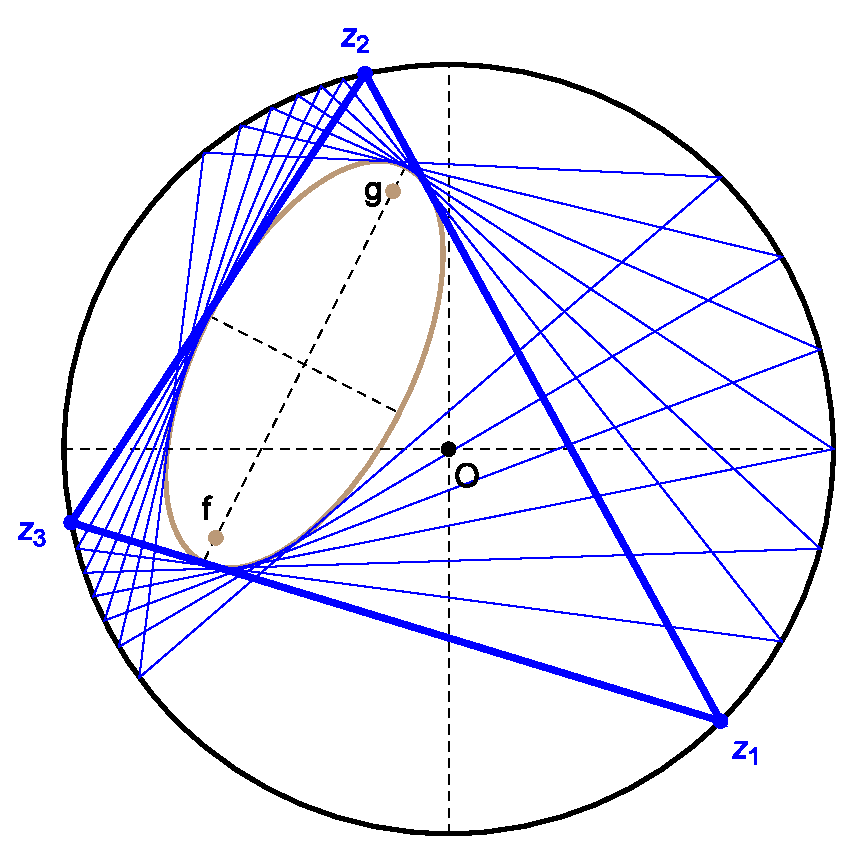
\includegraphics[width=.7\textwidth]{pics_03_050_blaschke_circum.eps}
    \caption{Blaschke complex parametrization of Poncelet 3-periodics (blue). Vertices are $z_1,z_2,z_3$. The foci of the caustic are $f,g$. }
    \label{fig:blaschke}
\end{figure}

%As a first step, identify points in $\R^2$ with points in the complex plane $\Cp$. Let $\D$ denote the open unit disk $\{z\in\Cp : |z|<1\}$ and $\T$ denote the unit circle $\{z\in\Cp : |z|=1\}$. By translation and scaling, we may assume the outer circle of the pair to be the unit circle $\T$. Let $\{f,g\}$ be the two foci of the inner ellipse.



Let  $\mathbb{T } = \{ z\in \mathbb{C}: |z| = 1\} $ the unit circle and $\mathbb{D} = \{ z\in\mathbb{C} : |z| < 1\} $ the open unit disk
bounded by $\mathbb{T }.$

Referring to \cref{fig:blaschke}, let $z_1,z_2,z_3\in\Cp$ denote the vertices of Poncelet 3-periodics in a generic $N=3$ family with fixed (unit) circumcircle denoted $\T=\{z\in\Cp : |z|=1\}$. Let $f,g$ be the foci of the caustic. Using Viète's formula, we obtain the following parametrization of the elementary symmetric polynomials on $z_1,z_2,z_3$ \cite{daepp-2019}:

\begin{definition}[Blaschke's Parametrization]
\begin{align*}
    \sigma_1:=z_1+z_2+z_3=& f+g+\l\ol f \ol g \\
    \sigma_2:=z_1 z_2+z_2 z_3+z_3 z_1=& f g+\l(\ol f+\ol g) \\
    \sigma_3:=z_1 z_2 z_3=& \l
\end{align*}
where $\l\in\T$ is the varying parameter.
\label{def:bla}
\end{definition}

\noindent Note that the concentric case occurs when $g=-f$.

For each $\l\in\T$, the three solutions of $B(z)=\l$ are the vertices of a 3-periodic orbit of the Poncelet family of triangles in the complex plane, \cite[Chapter 4]{daepp-2019}. Furthermore, as $\l$ varies in $\T$, the whole family of triangles is covered. Clearing the denominator in this equation and passing everything to the left-hand side, we get

\[
z^3-(f+g+\l\ol{f} \ol{g})z^2+(f g+\l(\ol f+\ol g))z-\l=0
\]

\begin{lemma}
If $u,v,w\in\mathbb{C}$ and $\lambda$ is a parameter that varies over the unit circle $\T\subset\mathbb{C}$, then the curve parametrized by
\[ F(\lambda)=u \lambda+ \frac{v}{\lambda}+w \]
is an ellipse centered at $w$, with semiaxis $|u|+|v|$ and $\big||u|-|v|\big|$, rotated with respect to the horizontal axis of $\mathbb{C}$ by an angle of $(\arg u+\arg v)/2$.
\label{lem:ell-param}
\end{lemma}

\begin{proof}
If either $u=0$ or $v=0$, the curve $h(\T)$ is clearly the translation of a multiple of the unit circle $\T$, and the result follows. Thus, we may assume $u\neq 0$ and $v\neq 0$.

Choose $k\in\mathbb{C}$ such that $k^2=u/v$. Write $k$ in polar form, as $k=r \mu$, where $r>0$ ($r\in\R$) and $|\mu|=1$. We define the following complex-valued functions:
\[R(z):=\mu z,~ S(z):=r z+(1/r) \ol{z},~ H(z):=k v z,~ T(z):=z+w\]

One can straight-forwardly check that $F=T\circ H\circ S\circ R$.

Since $|\mu|=1$, $R$ is a rotation of the plane, thus $R$ sends the unit circle $\T$ to itself. Since $r\in\R$, $r>0$, if we identify $\mathbb{C}$ with $\R^2$, $S$ can be seen as a linear transformation that sends $(x,y)\mapsto\left(\left(r+1/r\right)x,\left(r-1/r\right)y\right)$. Thus, $S$ sends $\T$ to an axis-aligned, origin-centered ellipse $\E_1$ with semiaxis $r+1/r$ and $|r-1/r|$. $H$ is the composition of a rotation and a homothety. $H$ sends the ellipse $\E_1$ to an origin-centered ellipse $\E_2$ rotated by an angle of $\arg(k v)=\arg(k)+\arg(v)=(\arg(u)-\arg(v))/2+\arg(v)=(\arg(u)+\arg(v))/2$. The semiaxis of $\E_2$ have length
\begin{align*}
|k v|&(r+1/r)=r|v|(r+1/r)=|r^2 v|+|v|=|k^2 v|+|v|=|u|+|v|\text{, and}\\
|k v|&|r-1/r|=r|v||r-1/r|=\big||r^2 v|-|v|\big|=\big||k^2 v|-|v|\big|=\big||u|-|v|\big|
\end{align*}

Finally, $T$ is a translation, thus $T$ sends $\E_2$ to an ellipse $\E_3$ centered at $w$, rotated by an angle $(\arg(u)+\arg(v))/2$ from the axis, with semiaxis lengths $|u|+|v|$ and $\big||u|-|v|\big|$, as desired.
\end{proof}

Consider the Moebius map $M_{z_0}=(z_0-z)/(1-\overline{z_0} z)$ and the Blaschke product of degree 3 given by   $B=M_{z_0} M_{z_1} M_{z_2}$.
\begin{theorem}
Let $B$ be a Blaschke product of degree 3 with
zeros $0, f, g.$ For $\lambda \in \mathbb{T}$, let $z_1, z_2, z_3 $ denote the three distinct solutions to $ B(z) = \lambda$. Then the
lines joining $z_j$ and $z_k$, $(j \ne k)$ are tangent to the ellipse given by
\[|w - f| + |w - g| = |1 -   \overline{f}   g |.\]
\end{theorem}
\begin{proof}
%\textcolor{red}{checar pagina}
See \cite[Theorem 2.9, page 37]{daepp-2019}.
\end{proof}

\begin{theorem}
 Given two points $f,g\in\mathbb{D}$. Then there exists a unique conic $\mathcal{E}$ with the foci
$f,g$   which is 3-Poncelet caustic with respect to $\mathbb{T}$. Moreover, $\mathcal{E}$ is an ellipse. That ellipse is
the Blaschke ellipse with the major axis of length $|1-\overline{f}g|.$
\end{theorem}

\begin{proof}
%\textcolor{red}{checar pagina}
See \cite[Corollary 4.4, page 44]{daepp-2019} and \cite{drag_milena2021}.
\end{proof}



